\begin{defproblem}{lp1:blocksworld1}%
 \begin{onlyproblem}%
	El mundo de los bloques consiste en un conjunto de bloques con forma de cubo situados en un tablero. Los bloques pueden ser amontonados, pero únicamente podemos situar uno sobre otro. Un brazo mecánico puede cambiar bloques de sitio, tanto sobre el tablero como sobre otros bloques. El brazo puede tomar sólo un bloque por cada instante de tiempo, de modo que no puede tomar uno si aún no ha soltado otro anterior. En la figura \ref{fig:ejemplo-bloques1} se puede ver un esquema de un mundo de los bloques posible.
	
	\begin{figure}[b]
		\centering
		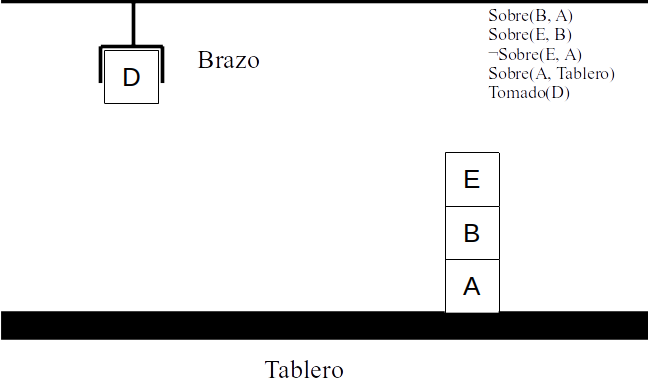
\includegraphics[width=0.7\linewidth]{Blocksworld-ejemplo}
		\caption[Mundo de los bloques de ejemplo]{Mundo de los bloques de ejemplo}
		\label{fig:ejemplo-bloques1}
	\end{figure}
	
	Sea $ B $ el conjunto formado por los bloques, y sea $ \mathcal{U} = B \cup \{tablero\} $ el dominio del discurso.
	
	Sea $ Sobre(x, y) $ el predicado que indica que el elemento $ x \in \mathcal{U} $ se encuentra inmediatamente sobre el elemento $ y \in \mathcal{U} $.
	
	Sea $ Tomado(b) $ el predicado que indica que el elemento $ b \in \mathcal{U} $ se encuentra tomado por el brazo.
	
	\begin{enumerate}
		\item Exprese utilizando Lógica de Predicados de Primer Orden que el elemento ``tablero'' no puede estar sobre otro elemento y que no puede estar tomado por el brazo.
		\item Para que el brazo mecánico pueda tomar un bloque es necesario que dicho bloque esté despejado (esto es, que no tenga ningún bloque sobre él) y que el brazo no esté sosteniendo algún bloque. Defina un predicado compuesto llamado $ PuedeTomar(x) $ que refleje este hecho.
		\item Evalúe la verdad o falsedad de los siguiente enunciados sobre el mundo de los bloques de la figura \ref{fig:blocksworld1}. Desarrolle la negación de cada uno de ellos.
		\begin{enumerate}
			\item $ \exists x, Sobre(A,x)  $
			\item $ \forall x, \forall y, Sobre(x,y) \land Sobre(y, x) \rightarrow x=y $
			\item $ \exists x, \forall y, x \neq y \rightarrow \neg Sobre(x, y) $
		\end{enumerate}
		\item Encuentre un dominio con al menos un bloque para que los siguientes enunciados sean verdaderos
		\begin{enumerate}
			\item $ \forall x, \neg PuedeTomar(x) $
			\item $ \exists x, \exists y, PuedeSoltar(x,y) \land y \neq Tablero $
			\item $ \forall x, \exists y,  x \neq Tablero \rightarrow Sobre(x, y) $
		\end{enumerate}
	\end{enumerate}

	\begin{figure}
		\centering
		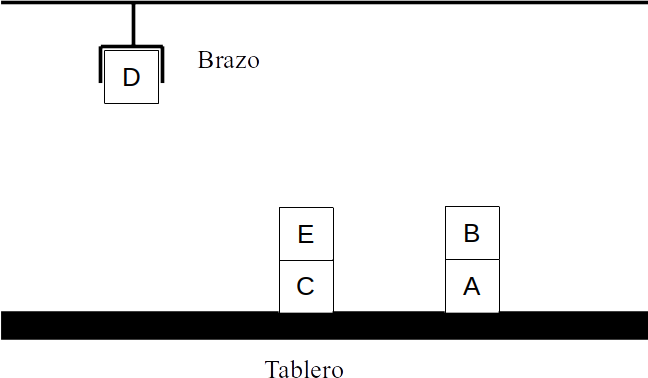
\includegraphics[width=0.7\linewidth]{Blocksworld1}
		\caption{Mundo de los bloques para el inciso c}
		\label{fig:blocksworld1}
	\end{figure}
	
 \end{onlyproblem}%
 \begin{onlysolution}%
 	
 	\end{onlysolution}
 \end{defproblem}
 

\begin{defproblem}{lp1:blocksworld2}%
	\begin{onlyproblem}%
		El mundo de los bloques consiste en un conjunto de bloques con forma de cubo situados en un tablero. Los bloques pueden ser amontonados, pero únicamente podemos situar uno sobre otro. Un brazo mecánico puede cambiar bloques de sitio, tanto sobre el tablero como sobre otros bloques. El brazo puede tomar sólo un bloque por cada instante de tiempo, de modo que no puede tomar uno si aún no ha soltado otro anterior. En la figura \ref{fig:ejemplo-bloques2} se puede ver un esquema de un mundo de los bloques posible.
		
		\begin{figure}[b]
			\centering
			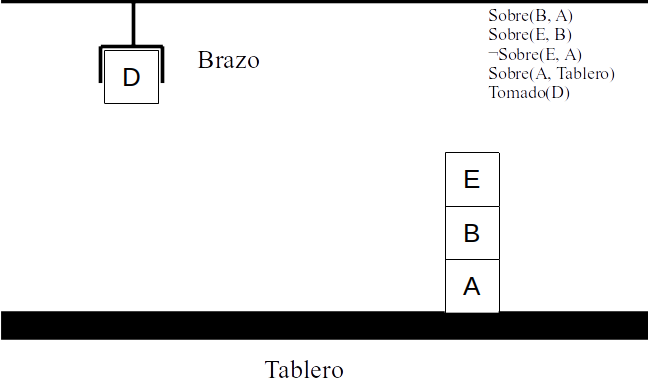
\includegraphics[width=0.7\linewidth]{Blocksworld-ejemplo}
			\caption[Mundo de los bloques de ejemplo]{Mundo de los bloques de ejemplo}
			\label{fig:ejemplo-bloques2}
		\end{figure}
		
		Sea $ B $ el conjunto formado por los bloques, y sea $ \mathcal{U} = B \cup \{tablero\} $ el dominio del discurso.
		
		Sea $ Sobre(x, y) $ el predicado que indica que el elemento $ x \in \mathcal{U} $ se encuentra inmediatamente sobre el elemento $ y \in \mathcal{U} $.
		
		Sea $ Tomado(b) $ el predicado que indica que el elemento $ b \in \mathcal{U} $ se encuentra tomado por el brazo.
		
		\begin{enumerate}
			\item Exprese utilizando Lógica de Predicados de Primer Orden que ningún elemento puede estar sobre sí mismo.
			\item El brazo mecánico puede soltar un bloque que esté sosteniendo sobre el tablero o sobre otro bloque, sólo cuando este último no tiene encima otro bloque. Defina un predicado compuesto $ PuedeSoltar(x,y) $ que refleje este hecho.
			\item Evalúe la verdad o falsedad de los siguiente enunciados sobre el mundo de los bloques de la figura \ref{fig:blocksworld2}. Desarrolle la negación de cada uno de ellos.
			\begin{enumerate}
				\item $ \neg \exists x, Tomado(x)  $
				\item $ \exists x, \exists y, Sobre(D,x) \land Sobre(x,y) $
				\item $ \exists x, \forall y, x \neq y \rightarrow \neg Sobre(y, x) $
			\end{enumerate}
			\item Encuentre un dominio con al menos un bloque para que los siguientes enunciados sean verdaderos
			\begin{enumerate}
				\item $ \exists x, \neg Tomado(x) \land \neg Sobre(x, Tablero) $
				\item $ \exists x, \exists y, Tomado(x) \land \neg PuedeSoltar(x,y) $
				\item $ \exists x, \forall y, Tomado(x) \land (x \neq y \rightarrow PuedeSoltar(x,y)) $
			\end{enumerate}
		\end{enumerate}
	
		\begin{figure}
			\centering
			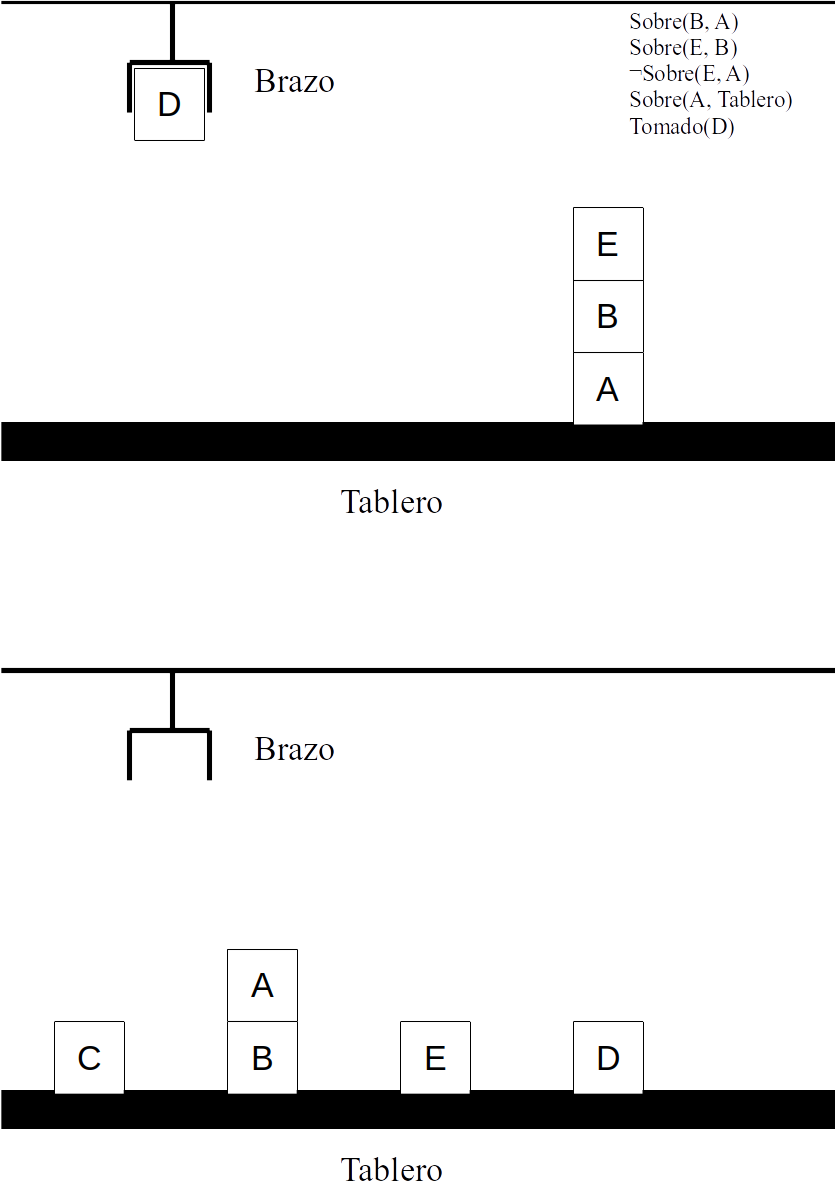
\includegraphics[width=0.7\linewidth]{Blocksworld2}
			\caption{Mundo de los bloques para el inciso c}
			\label{fig:blocksworld2}
		\end{figure}
	\end{onlyproblem}%
	\begin{onlysolution}%
		
	\end{onlysolution}%
\end{defproblem}

\begin{defproblem}{lp1:blocksworld3}%
	\begin{onlyproblem}%
		El mundo de los bloques consiste en un conjunto de bloques con forma de cubo situados en un tablero. Los bloques pueden ser amontonados, pero únicamente podemos situar uno sobre otro. Un brazo mecánico puede cambiar bloques de sitio, tanto sobre el tablero como sobre otros bloques. El brazo puede tomar sólo un bloque por cada instante de tiempo, de modo que no puede tomar uno si aún no ha soltado otro anterior. En la figura \ref{fig:ejemplo-bloques3} se puede ver un esquema de un mundo de los bloques posible.
		
		\begin{figure}[b]
			\centering
			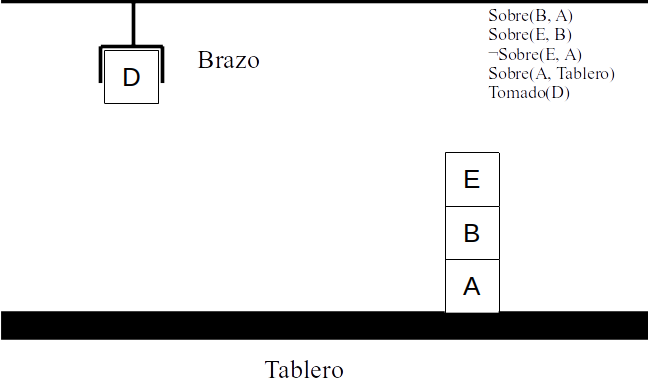
\includegraphics[width=0.7\linewidth]{Blocksworld-ejemplo}
			\caption[Mundo de los bloques de ejemplo]{Mundo de los bloques de ejemplo}
			\label{fig:ejemplo-bloques3}
		\end{figure}
		
		
		Sea $ B $ el conjunto formado por los bloques, y sea $ \mathcal{U} = B \cup \{tablero\} $ el dominio del discurso.
		
		Sea $ Sobre(x, y) $ el predicado que indica que el elemento $ x \in \mathcal{U} $ se encuentra inmediatamente sobre el elemento $ y \in \mathcal{U} $.
		
		Sea $ Tomado(b) $ el predicado que indica que el elemento $ b \in \mathcal{U} $ se encuentra tomado por el brazo.
		
		\begin{enumerate}
			\item Exprese utilizando Lógica de Predicados de Primer Orden que si hay un elemento que no está sobre ningún otro, entonces o bien es el tablero o bien está tomado por el brazo
			\item Defina un predicado compuesto llamado $ Despejado(x) $ que sea verdadero si y sólo si $ x \in B $ no tiene ningún bloque sobre sí mismo o es el tablero, que está siempre despejado.
			\item Evalúe la verdad o falsedad de los siguiente enunciados sobre el mundo de los bloques de la figura \ref{fig:blocksworld3}. Desarrolle la negación de cada uno de ellos.
			\begin{enumerate}
				\item $ \forall x, Tomado(x) \rightarrow \neg Sobre(x, Tablero) $
				\item $ \exists x, \exists y, Sobre(D,x) \land Sobre(x,y) $
				\item $ \forall x, \exists y, \neg Sobre(y, x) \rightarrow y \neq Tablero $
			\end{enumerate}
			\item Encuentre un dominio con al menos un bloque para que los siguientes enunciados sean verdaderos
			\begin{enumerate}
				\item $ \forall x, \neg PuedeSoltar(x, Tablero) $
				\item $ \exists x, \exists y, Tomado(x) \land \neg PuedeSoltar(x,y) $
				\item $ \forall x, \exists y,  x \neq Tablero \rightarrow Sobre(x, y) $
			\end{enumerate}
		\end{enumerate}
		
		\begin{figure}
			\centering
			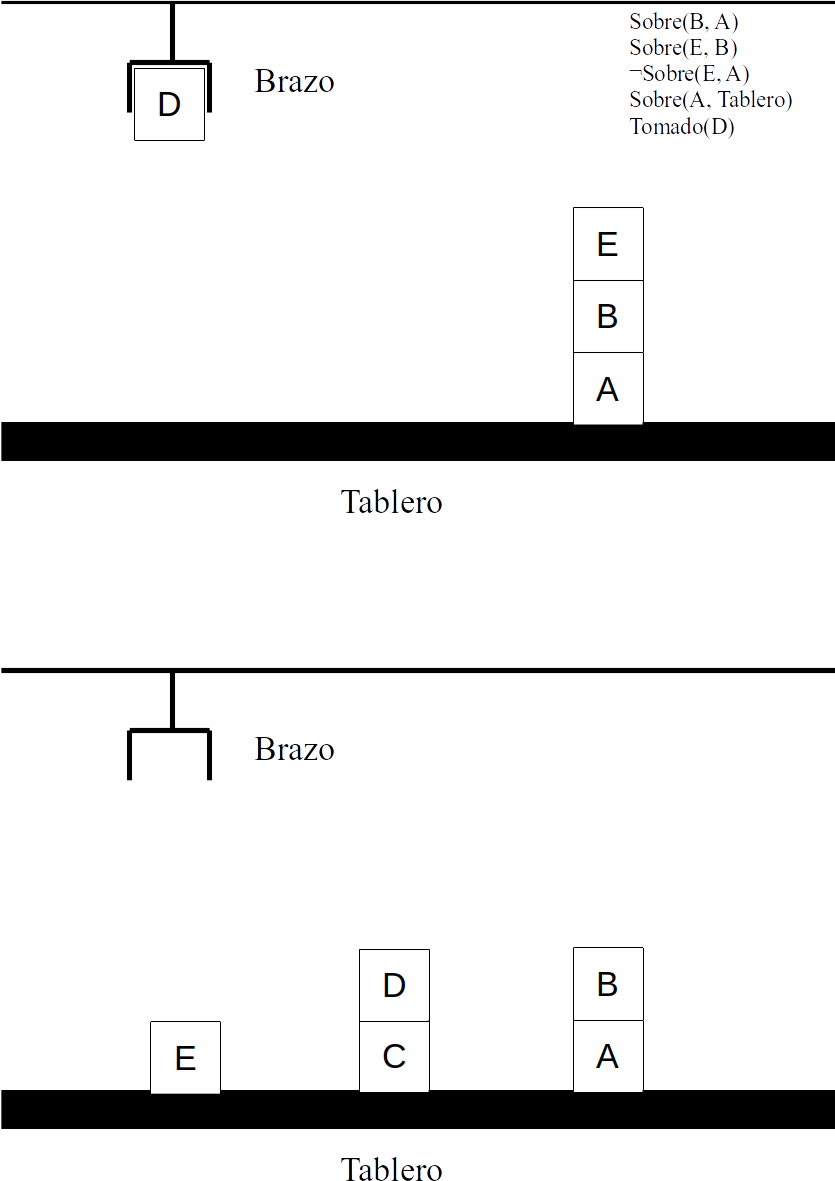
\includegraphics[width=0.7\linewidth]{Blocksworld3}
			\caption{Mundo de los bloques para el inciso c}
			\label{fig:blocksworld3}
		\end{figure}
	
	\end{onlyproblem}%
	\begin{onlysolution}%
		
	\end{onlysolution}%
\end{defproblem}

\begin{defproblem}{lp1:blocksworld4}%
	\begin{onlyproblem}%
		El mundo de los bloques consiste en un conjunto de bloques con forma de cubo situados en un tablero. Los bloques pueden ser amontonados, pero únicamente podemos situar uno sobre otro. Un brazo mecánico puede cambiar bloques de sitio, tanto sobre el tablero como sobre otros bloques. El brazo puede tomar sólo un bloque por cada instante de tiempo, de modo que no puede tomar uno si aún no ha soltado otro anterior. En la figura \ref{fig:ejemplo-bloques4} se puede ver un esquema de un mundo de los bloques posible.
		
		\begin{figure}[b]
			\centering
			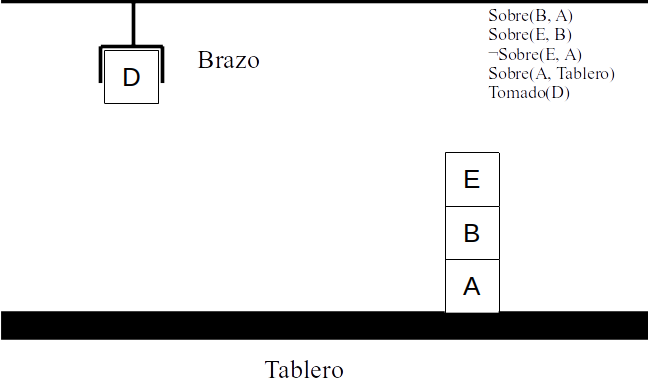
\includegraphics[width=0.7\linewidth]{Blocksworld-ejemplo}
			\caption[Mundo de los bloques de ejemplo]{Mundo de los bloques de ejemplo}
			\label{fig:ejemplo-bloques4}
		\end{figure}
		
		
		Sea $ B $ el conjunto formado por los bloques, y sea $ \mathcal{U} = B \cup \{tablero\} $ el dominio del discurso.
		
		Sea $ Sobre(x, y) $ el predicado que indica que el elemento $ x \in \mathcal{U} $ se encuentra inmediatamente sobre el elemento $ y \in \mathcal{U} $.
		
		Sea $ Tomado(b) $ el predicado que indica que el elemento $ b \in \mathcal{U} $ se encuentra tomado por el brazo.
		
		\begin{enumerate}
			\item Exprese utilizando Lógica de Predicados de Primer Orden que no puede haber dos elementos distintos tomados por el brazo.
			\item Para que el brazo mecánico pueda tomar un bloque es necesario que dicho bloque esté despejado (esto es, que no tenga ningún bloque sobre él) y que el brazo no esté sosteniendo algún bloque. Defina un predicado compuesto llamado $ PuedeTomar(x) $ que refleje este hecho.
			\item Evalúe la verdad o falsedad de los siguiente enunciados sobre el mundo de los bloques de la figura \ref{fig:blocksworld4}. Desarrolle la negación de cada uno de ellos.
			\begin{enumerate}
				\item $ \exists x, Sobre(A,x)  $
				\item $ \forall x, \neg (\exists y, Sobre(x,y)) \rightarrow Tomado(x) $
				\item $ \exists x, \forall y, x \neq y \rightarrow \neg Sobre(y, x) $
			\end{enumerate}
			\item Encuentre un dominio con al menos un bloque para que los siguientes enunciados sean verdaderos
			\begin{enumerate}
				\item $ \exists x, \neg Sobre(x, Tablero) \land \neg PuedeTomar(x) \land Despejado(x) $
				\item $ \exists x, \exists y, Tomado(x) \land \neg PuedeSoltar(x,y) $
				\item $ \exists x, \forall y, Tomado(x) \land (x \neq y \rightarrow PuedeSoltar(x,y)) $
			\end{enumerate}
		\end{enumerate}
		
		\begin{figure}
			\centering
			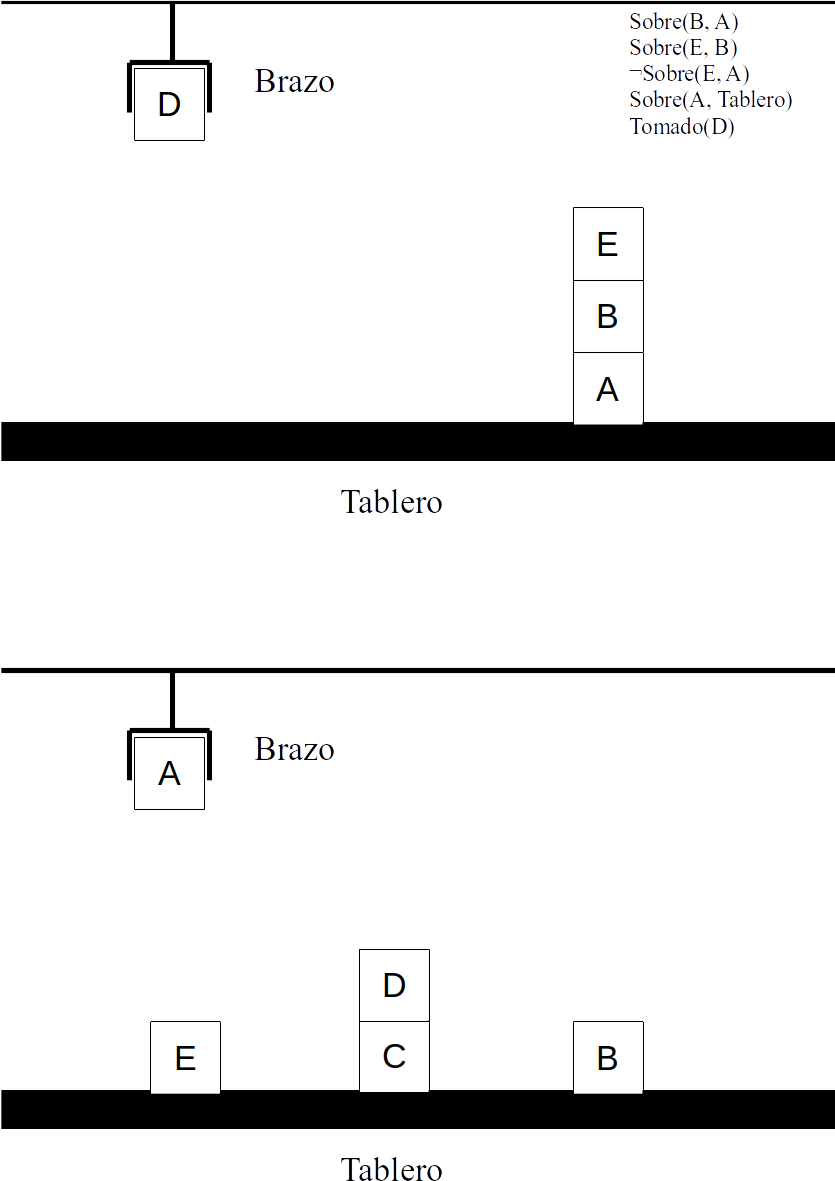
\includegraphics[width=0.7\linewidth]{Blocksworld4}
			\caption{Mundo de los bloques para el inciso c}
			\label{fig:blocksworld4}
		\end{figure}
	
	\end{onlyproblem}%
	\begin{onlysolution}%
		
	\end{onlysolution}%
\end{defproblem}